% FUNDAMENTAÇÃO TEÓRICA--------------------------------------------------------

\chapter{FUNDAMENTAÇÃO TEÓRICA}
\label{chap:fundamentacaoTeorica}

As grandes habilidades do ser humano, como a capacidade de aprendizado e de realizar funções complexas, motivam muitos pesquisadores a investigar o funcionamento do cérebro e desenvolverem técnicas que possibilitem reproduzir suas
funções (FERNEDA, 2006). Motivados a tornar possível que computadores executem tarefas consideradas complexas, ao longo dos anos, foram propostos diversos algoritmos capazes de realizar tarefas como reconhecimento de sinais de áudios e imagens, tomada de decisão, entre outros, de maneira eficaz e eficiente. Paradigmas que buscam reproduzir as funções do cérebro humano compreendem a área de Inteligência Artificial – IA – da ciência da computação.

\section{APRENDIZADO DE MÁQUINA}
\label{sec:titSecAprenMaquina}

Aprendizado de máquina – AM – é uma subárea de grande importância da Inteligência Artificial, pois o aprendizado é um fator fundamental para um comportamento inteligente (BATISTA, 2003, p. 39). A construção do seu modelo matemático foi baseado no funcionamento dos neurônios do cérebro dos vertebrados, o qual denomina-se pela técnica computacional de Rede Neural Artificial, que adquirem conhecimento com base em experiências, melhorando gradualmente sua capacidade de desempenho.

O AM tem o objetivo de construir programas computacionais que sejam capazes de obter conhecimento de maneira autônoma, ou seja, desenvolver sistemas que baseiam tomadas de decisões em experiências adquiridas anteriormente, por meio de resoluções bem sucedidas de problemas semelhantes (MONARD; BARANAUSKAS, 2003).

O uso de algoritmos de aprendizado permitiu que diversas tarefas complexas fossem possíveis de serem realizadas e até superar os resultados obtidos por humanos. Um exemplo é um algoritmo de aprendizado de máquina, desenvolvido por Silver et al. (2016), que venceu o campeão mundial do jogo \textit{Go}, um dos jogos estratégicos mais antigos do mundo que possui uma alta complexidade e uma infinidade de possibilidades de jogadas.

O algoritmo de AM também permitiu que tarefas complexas ou exaustivas para o humano fossem realizadas de forma eficiênte. Como em Souto et al. (2003), por exemplo, um algoritmo de aprendizado de máquina foi utilizado para realizar a análise de dados biológicos, dada a restrição da análise manual diante do número de dados biológicos que aumenta exponencialmente a cada ano.


\subsection{APRENDIZADO SUPERVISIONADO}
\label{sec:titSecAprenSupervisionado}

A indução é um conceito que caracteriza a forma de obter conclusões genéricas com base em exemplos específicos, em outras palavras, o aprendizado ocorre à partir de uma inferência em padrões apresentados. A indução é umas das principais formas de derivar conhecimento novo, foi com ela que as principais descobertas do mundo tornaram-se conhecidas. Embora a indução seja uma das principais maneiras do cérebro humano converter exemplos em conhecimento, deve-se ter cuidado ao utilizá-la, pois com padrões insuficientes ou mal escolhidos levam a uma inferência incorreta (MONARD; BARANAUSKAS, 2003, cap. 4).	

Além de uma subárea do aprendizado de máquina, existem duas vertentes básicas de aprendizado indutivo, o aprendizado supervisionado e o não supervisionado. O presente trabalho abordou o aprendizado supervisionado.

O aprendizado supervisionado, ou indutor, consiste em apresentar a um algoritmo dados de treinamento que representam alguns padrões de entrada e seus respectivos padrões de saída esperados, ou seja, o algoritmo conhece a priori o rótulo de todo o conjunto de dados de treinamento (BLASCHKO; KUMAR; TASKAR, 2013). Dessa forma, o mesmo consegue, a partir de tais dados construir um modelo de aprendizado capaz de ser utilizado posteriormente para rotular amostras desconhecidas (i.e. amostras de teste). Recentemente, o aprendizado supervisionado baseado em arquiteturas de redes neurais profundas, ressurgiu apresentando resultados notáveis quando aplicados a problemas que envolvam visão computacional e análise de imagens, sendo utilizado em aplicações como classificação de imagens e/ou detecção de objetos (KRIZHEVSKY; SUTSKEVER; HINTON, 2012).


\subsection{APRENDIZADO PROFUNDO}
\label{sec:titSecAprenProfundo}

Aprendizado profundo, do inglês \textit{Deep Learning} (DL), é uma subárea do aprendizado de máquina que explora o processamento de informações em diversos estágios, com o objetivo de classificar padrões e realizar a aprendizagem de recurso ou representação (WAN et al., 2014). A modelagem do problema de reconhecimento é feita por meio de um grafo ponderado em camadas, cada camada possui um conjunto de características abstratas que são conectadas as características das demais camadas (CHEN et al., 2015).

As principais áreas de pesquisa do aprendizado profundo são no desenvolvimento de técnicas capazes de reproduzir alguns comportamentos humanos, como processamento de linguagem natural, reconhecimento visual e reconhecimento da fala. A DL é muito utilizada nessas áreas por ser uma tecnologia que possibilita aprendizado ininterrupto, semelhante ao cérebro humano, além de possuir grande flexibilidade e capacidade de processamento de informações complexas. Comparada a outras metodologias clássicas de aprendizado de máquina, o aprendizado profundo oferece grandes vantagens, podendo superar a capacidade humana, principalmente na resolução de problemas com um grande volume de dados não estruturado. Isso ocorre devido ao fato do seu modelo matemático ser mais flexível, isso possibilita que os \textit{inputs} sejam definidos pelo modelo, no qual analisa todos os parâmetros de entrada e decide quais trarão os melhores resultados (FERNANDES; SILVA, 2017).

LeCun et al. (2015) acreditam que em um futuro próximo o aprendizado de máquina será cada vez mais utilizado por demandar pouco trabalho manual para a sua construção, podendo usufruir de uma melhor maneira da capacidade computacional e de dados.

\section{IMAGENS NA VISÃO COMPUTACIONAL}
\label{sec:titSecVisaoComputacional}

A visão computacional tornou-se grande aliada para solucionar problemas do homem. Um grande exemplo são os radares fixos de velocidade, quando um carro cruzar entre os sensores localizados no asfalto, acima de uma velocidade pré-determinada, é acionada uma câmera, essa câmera captura uma imagem da placa traseira de um automóvel e em seguida é identificado cada caractere da placa. Todo o processo de identificar uma placa na traseira de um automóvel e reconhecer os sete caracteres da placa envolve processamento digital de imagem.

Processamento Digital de Imagens (PDI) trata-se de processar sinais com o intuito de extrair mais facilmente as informações contida (ALBUQUERQUE, 2003). O processamento envolve algumas etapas, como: aquisição da imagem, pré-processamento, segmentação, representação e descrição, e reconhecimento e interpretação (PEDRINI; SCHWARTZ, 2008).

A etapa de aquisição, como o próprio nome induz, refere-se a adquirir uma imagem. O pré-processamento refere-se à algumas técnicas que serão empregadas na imagem de modo a obter melhores resultados na extração das informações desejadas, por exemplo, na \autoref{fig:figura-exemploPreProcessamento} (a) apresenta um raio-x com pouca visibilidade dos ossos presentes  e (b) a imagem após aplicação do filtro de equalização de histograma. O processo de segmentação objetiva extrair os objetos de interesse da imagem, frequentemente usada para remoção de fundos. Em representação e descrição serão extraídas atributos da imagem, essa etapa é caracterizada pela rotulação, onde será atribuído uma \textit{label} que poderá indicar a qual classe a imagem pertence; e pela extração de atributos onde será reunido um conjunto de características, representadas numericamente, que podem descrever cores, texturas, formas, entre outras.  A última etapa, reconhecimento e interpretação, objetiva realizar de, maneira automática, a identificação dos objetos segmentados. Nessa última etapa é comum o uso de uma sub-área da IA, o aprendizado de máquina, pela necessidade de realizar um aprendizado e uma representação dos padrões aprendidos (ALBUQUERQUE, 2003).


\begin{figure}[!htb]
    \centering
    \caption{Exemplo de pré-processamento}
    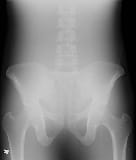
\includegraphics[width=0.3\textwidth]{./dados/figuras/figura1-a.jpg}
    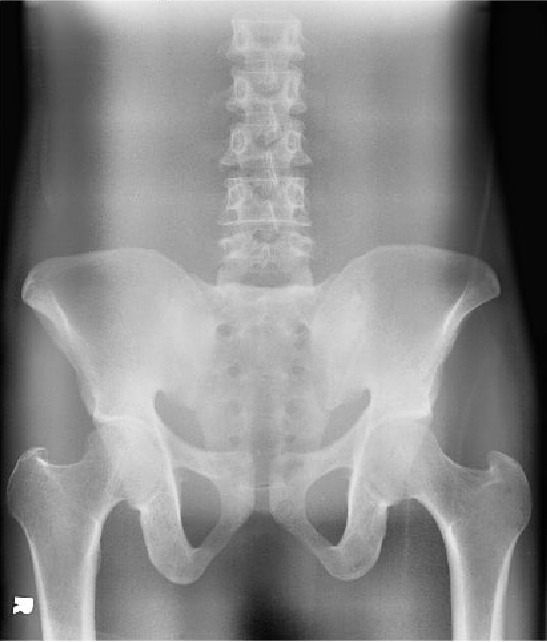
\includegraphics[width=0.3\textwidth]{./dados/figuras/figura1-b.jpeg}
    \fonte{Adaptado de}
    \label{fig:figura-exemploPreProcessamento}
\end{figure}


\section{ANÁLISE DE SEMENTES}
\label{sec:titSecAnalSementes}

O Brasil é o maior produtor e exportador de soja do mundo, são inúmeras as vantagens que o levaram a essa posição, como a alta capacidade do grão em se adaptar a diferentes tipos de solo e clima. Isso exige que a produção seja sempre de alta qualidade, garantir um alto vigor à soja garante que o grão possa tolerar facilmente mudanças climáticas, doenças e pragas, por exemplo (HORIKOSHI et al., 2018).

Existem diversos testes e experimentos em laboratórios que pesquisam e aplicam técnicas para evolução da qualidade do grão. Um teste em destaque é o teste de tetrazólio, um método de controle de qualidade, com alta precisão, rapidez e possibilidade de extrair uma grande quantidade de informações. O teste permite verificar o vigor do grão de soja e possíveis causas que o levaram a ter o vigor reduzido, como dano por excesso de umidade, danos mecânicos ou danos causados por percevejos (PAGLIONE, 2016).

\begin{figure}[!htb]
    \centering
    \caption{Sementes submetidas ao teste de tetrazólio}
    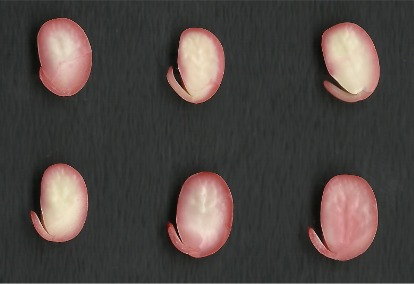
\includegraphics[width=0.5\textwidth]{./dados/figuras/soybean.jpeg}
    \fonte{(SANTANNA et al., 2014)}
    \label{fig:figura-sojasTeste}
\end{figure}

O teste consiste em aplicar uma solução em uma amostra de sementes, que foram previamente cortadas longitudinal e medianamente, no sentido do comprimento, selecionando a metade mais apropriada ao teste (OLIVEIRA, 2009). A solução do teste proporciona aos grãos amostras uma cor avermelhada, segundo França Neto et al. (1998), as diferentes cores observadas são características que são consideradas nos resultados do teste. Por exemplo, a cor rosa claro sinaliza uma semente de alto vigor, por outro lado, sementes que apresentam uma cor rosa escuro apresentam tecido em deterioração.

